% Title: Report LaTex File: Literature Review
% Auther: DC Eksteen
% Student Number: 22623906
% Contact: 22623906@sun.ac.za
% Date: 2022/09/17
% Version: 2.1

\chapter{Literature Review}
\label{sec:lit}
% Overview of the focus of the lietrature review:

% Plan for Literature Review Layout:
% Zwift: Technology and Requirements
% Existing Trainer Technology
% Bluetooth Technology
% Bicycle Specifications
% Eddy Current Brake
% Sensor Technology

The literature review is performed to demonstrate the investigation and refinement of the technical requirements for compatibility with Zwift and the training platform that was subsequently developed. These technical requirements are then refined into engineering and functional requirements in Section \ref{sec:req}.

The review starts by investigating the utilization of Zwift and to identify the requirements to achieve this. Any identified technology or information that requires further investigation is then analysed and reviewed in subsequent sections of the review.

The review then continues to investigate and identify the technical requirements of the training platform that was developed. This is achieved by identifying and investigating commonly used products and technology offered on the market.

\newpage

\section{Zwift Technical Requirements}

\subsection{Basic Requirements}
As mentioned in the introduction, Zwift utilizes real-time training data provide instant feedback to the user in the form of a digital avatar moving in a virtual environment. Zwift works similar to modern multilayer computer games, where the game is hosted on a centralised server, and users connect to this server(s) through the internet using an \ac{api} integrated into a downloadable application.

The application is available from the official website, and is available for download on Mac, Windows, Android and iOS. The application requires a user account that can be created as a free trial version, or after the trail period as a paid subscription. The device that Zwift will be installed on is required to connect to an external trainer or sensors using either \acs{ble} or ANT+, and the device should thus support this technology. \citep{Zwift:2022}

\begin{figure}[H]
	\begin{center}
		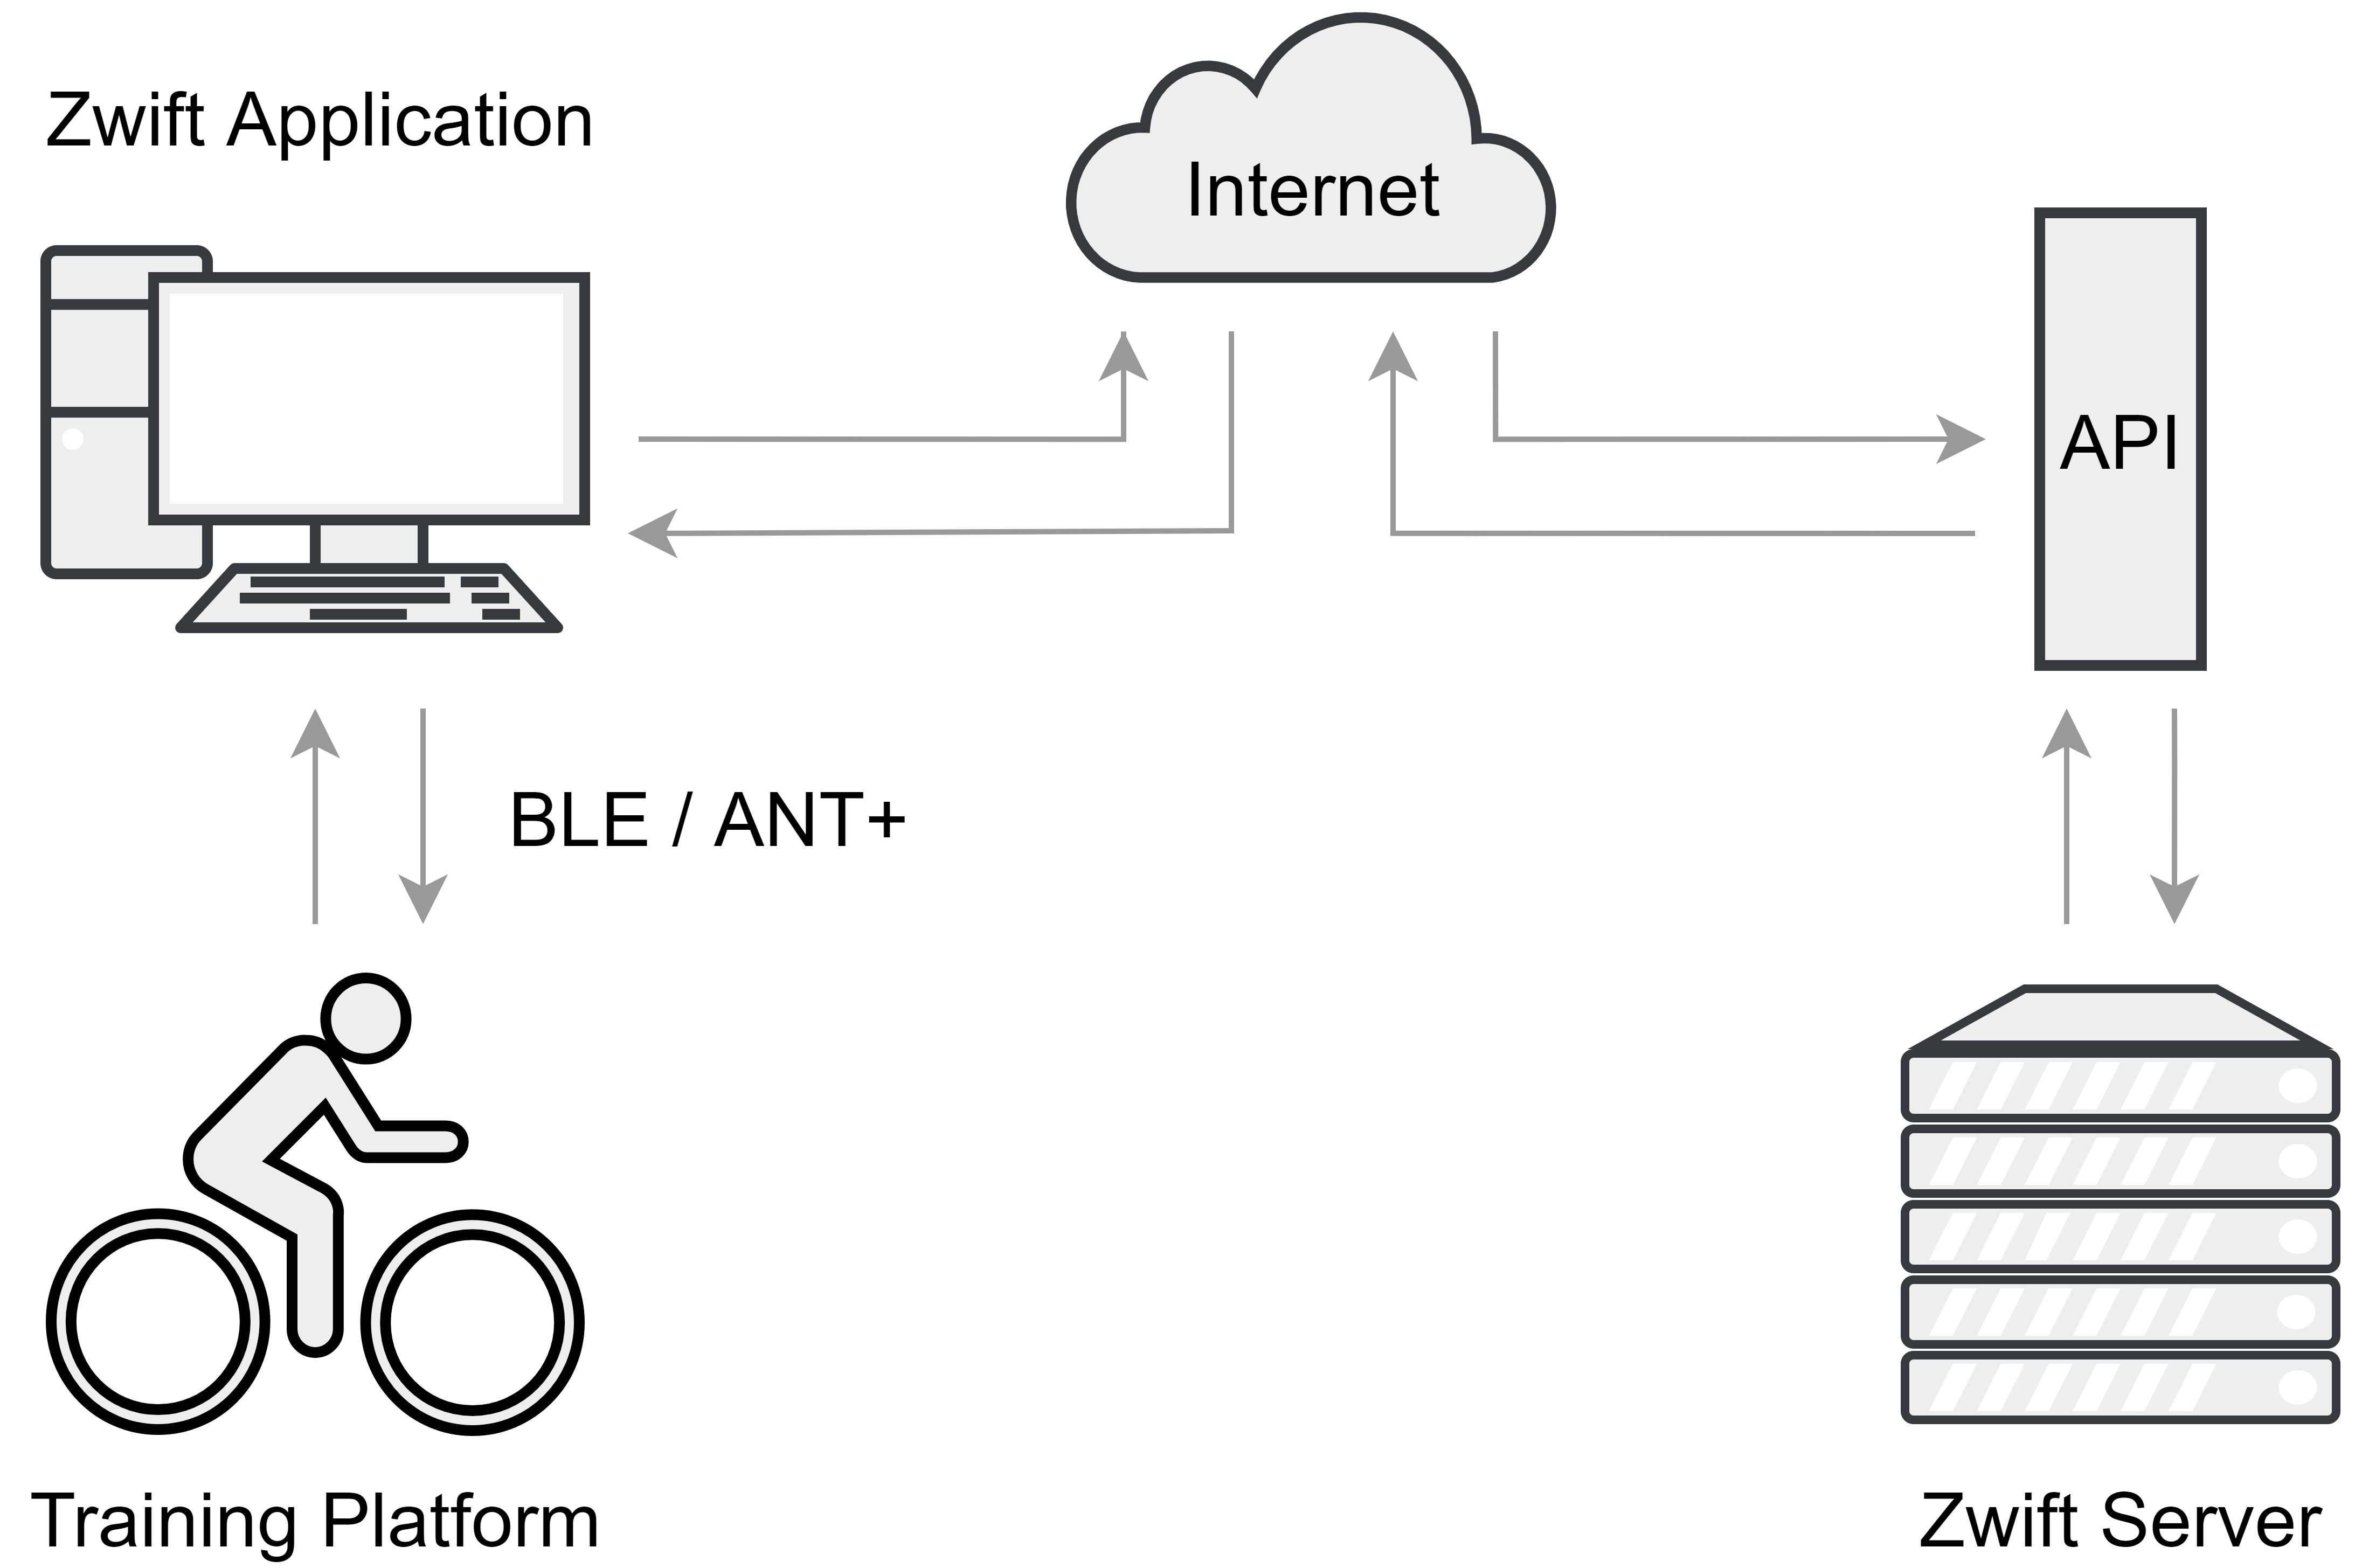
\includegraphics[width=0.7\textwidth]{ZwiftConnection.jpg}
		\caption{Zwift Connection Overview}
		\label{fig:zwift}
	\end{center}
\end{figure}

Figure \ref{fig:zwift} shows an overview of the connections that are required while using the Zwift application. This project will mainly focus on the training platform and the communication with the Zwift application.

\subsection{Training Platform Requirements}
The Zwift application provides support for many different training platform types as well as independent sensors to be used as input devices. The main types of configuration that are described on the official website are: wheel-on trainers, direct drive trainers and smart bikes. These were investigated in more depth in Section \ref{sec:train}.

The training platform serves three main purposes: to facilitate the training session by providing the cyclist with a means of cycling, to measure, process and transmit the data that is required by Zwift and to adjust the training experience based on feedback from the Zwift application. As shown in Figure \ref{fig:zwift}, the training platform sends and receives data from the device where the Zwift application is installed and running. This is achieved using \ac{ble} or ANT+ technology.

If the connected training platform utilizes ANT+, the \ac{fec} protocol is implemented for communication, where a \ac{ble} connection will utilize the \ac{ftms} protocol. These are investigated in more depth in section \ref{sec:ant}. The Zwift application also provides the option to connect to speed, cadence and power sensors in addition to smart trainers. The supported and required measurement data are explained in the following subsections.

\subsubsection{Cycling Power}
The most important parameter that is required for experiencing the Zwift application is the Power input by the cyclist. This can be measured using power sensors, or calculated from other measurements. Power sensors measure the input force provided by the user, and multiply this by the cadence to find the input power using equation \ref{eq:pow}. If the input force is not known, but the braking force can be determined and the wheel speed is known, then the power can still be calculated using equation \ref{eq:pow}. This is called simulated power, and is what Zwift uses when it does not receive direct power measurements.

\begin{equation}
	P = \acs{omega} \times \acs{T}
	\label{eq:pow}
\end{equation}

\subsubsection{Cycling Speed}
Cycling speed is the speed at which the cyclist would be travelling if they were not fixed to the training platform. It can be calculated by measuring the wheel rotational speed and wheel diameter using equation \ref{eq:spd}, where $D$ is the diameter of the wheel.

\begin{equation}
	\acs{v} = \acs{omega} \times \frac{D}{2}
	\label{eq:spd}
\end{equation}

Zwift uses the speed measurement of the cyclist to control the speed of the avatar in the virtual environment. This is thus the most basic type of data that is required to interact with the application. If a supported "dumb" or turbo trainer is used, then Zwift can determine the braking force that is applied given curtain conditions such as brake lever position and riding speed.
The minimum requirement for full utilization of the platform is a speed sensor when using a supported wheel-on trainer.

\subsubsection{Cycling Cadence}
Cadence is the rotation rate of the pedals of the bike and is usually measured in \ac{rpm}. Zwift does not require any cadence data for interacting with the platform, as it does not take the cadence into account for controlling the virtual avatar. Cadence data is often used by cyclists as a gauge of how hard the given exercise is. A higher cadence means that the cyclists is cycling faster and experiencing a more intense workout, where a slower cadence might mean that there is more load on the cyclists legs, but at a lower intensity.



\section{\ac{ble} vs ANT+}
\label{sec:ant}

\ac{ble} and ANT+ are wireless communication technologies that are both widely used in consumer products across many industries. Both \ac{ble} and ANT+ devices communicate over \ac{uhf} electromagnetic waves with frequencies around \SI{2.4}{\giga\hertz}. This communication takes place over small distances and requires both transmitting and receiving device to have supporting hardware in order to communicate.

\subsection{ANT+ \acl{fec}}

ANT+ was developed and marketed by ANT Wireless. It is a sensor network technology that allows for communication between sensors and monitors, and is primarily used for activity tracking. The propriety nature of the ANT+ technology meaning that a specific ANT+ dongle is required for implementation makes this protocol less ideal for this project as it limits the accessibility of some possible future development and implementation.

The ANT+ \ac{fec} protocol was developed specifically for smart training equipment from the ground up, and thus provides a good low energy solution to many manufacturers. The \ac{fec} protocol is the only ANT+ protocol that is supported by the Zwift application at the time of writing. ANT+ hardware is required by both the device where Zwift is installed, as well as the training platform.

\subsection{\ac{ble} for Fitness Devices}
\ac{ble} is one of two standards for Bluetooth communication that has been developed and is maintained by \ac{bsig}.\footnote{Other standard being Bluetooth \ac{bbr}} The specific details of the technology and standard is discussed in Section \ref{sec:ble}. For the sake of Zwift requirements, this section will look at the specific protocol of the \ac{ble} specification that Zwift supports.

When Zwift was initially launched, all of the Bluetooth communication was performed using proprietary protocols provided by the manufacturers of trainers and training equipment as there has not yet been a standard protocol defined to specify Bluetooth communication of controllable sports equipment.

On 14 February 2017, \ac{bsig} adopted the \ac{ftms} protocol to the \ac{ble} \ac{gatt}. Then, in late 2021 Zwift announced that they will be supporting \ac{ftms} in their latest update, and thus any new trainer that would like to interact with the Zwift platform would be required to follow the \ac{ftms} protocol as is discussed in Section \ref{sec:ftms}. \citep{Jeremy:2021}\\

Zwift does not implement the full \ac{ftms} protocol, as this would add unnecessary complexity to equipment manufacturers. Table \ref{tab:blreq} below shows the different commands within the \ac{ftms} protocol that Zwift uses to control connected trainers. This was deducted from the control modes that are available on the platform, and have been confirmed by a Zwift engineer on the official support forums. \citep{Jeremy:2021}

\begin{table}[H]
	\renewcommand{\arraystretch}{\tablestretch}
	\centering
	\caption{Zwift Supported \ac{ftms} Commands}
	\begin{tabularx}{\textwidth}{ >{\raggedright}p{4cm} X}
		\toprule
		Command          & Description                                                              \\
		\midrule
		Resistance Level & Sends the desired resistance level to the trainer                        \\
		Target Power     & Sends the targeted power (Watts) that the trainer should aim to maintain \\
		Start or Resume  & Starts or resumes a training session on the trainer                      \\
		Stop or Pause    & Stop or pause a training session on the trainer                          \\
		\ac{sim}         & Set the simulation parameters on the trainer                             \\
		\bottomrule
	\end{tabularx}
	\label{tab:blreq}
\end{table}

Zwift will use the commands above to control the training platform depending on the mode that is set and used within the application. The two main modes that can be chosen within Zwift is the \acf{erg} mode or \acf{sim} mode. \ac{erg} stems from the Greek word "Ergasia", which means "work", and is implemented using the Target Power command and requires the training platform to adjust the resistance in reaction to the rider speed in order to maintain the target power level. \citep{Zwiftinsider:2022}

\ac{sim} mode utilizes a separately defined control point within the \ac{ftms} standard and is investigated in more detail in section \ref{sec:sim}.

Lastly, the user can adjust the resistance on their trainer from within the Zwift software, enabling Zwift to then send that specific command to the trainer when the user would like to change the immediate resistance level.

\section{\ac{ble} Communication}
\label{sec:ble}

\ac{ble} works by forming pico - and scatternet networks between various master and slave devices. Each device in the network is either a master or a slave, but never both. The devices then form a piconet when one or more slaves connect and synchronize with a single master device. The role of the master device is then to manage the slave devices through the protocol. This forms a 'star' network topology which is illustrated in Figure \ref{fig:ble}. \citep{Townsend:2014}

\begin{figure}[H]
	\begin{center}
		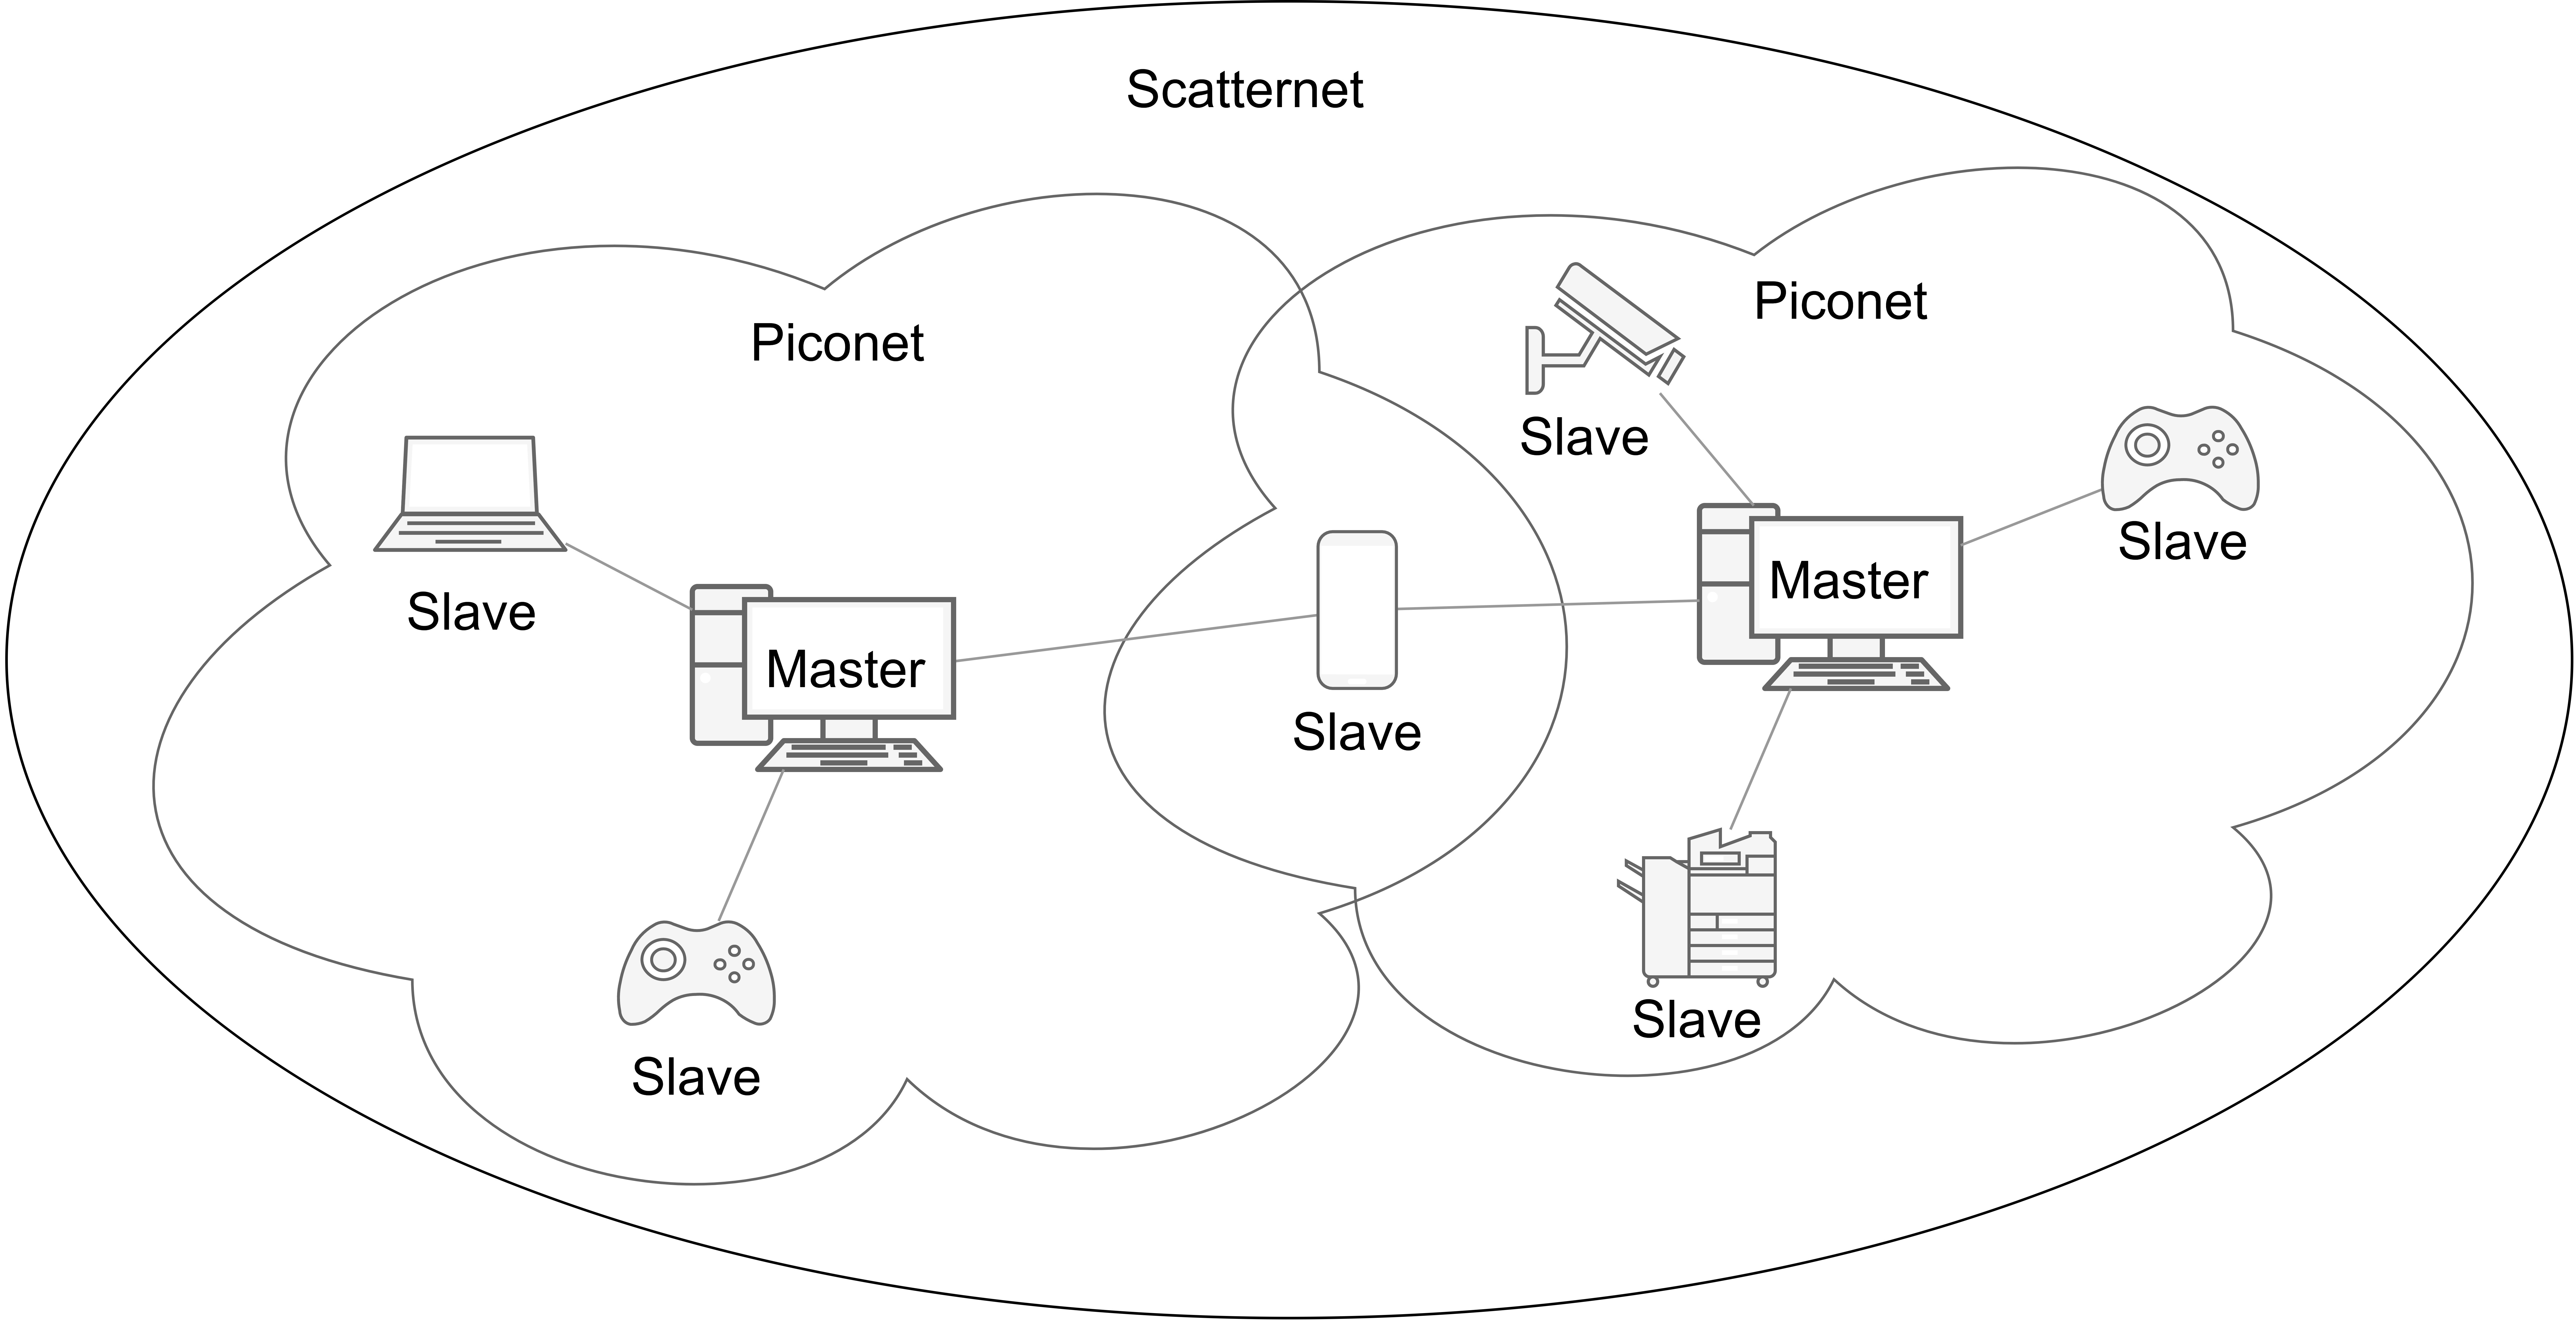
\includegraphics[width = \textwidth]{BLEnet.jpg}
		\caption{\ac{ble} Star Network Topology}
		\label{fig:ble}
	\end{center}
\end{figure}

Specifications from the \ac{ble} specification sheet is shown in Table \ref{tab:ble}. The \ac{ble} protocol is divided into various standardized and proprietary profiles that specify specific communication architectures. The \aca{gatt} profile is used by \ac{bsig} to standardize various common service applications, and is also the profile where the \ac{ftms} service that is required by Zwift is specified.

\begin{table}[H]
	\renewcommand{\arraystretch}{\tablestretch}
	\centering
	\caption{Technical Specifications of the \ac{ble} Standard}
	\begin{tabularx}{\textwidth}{>{\raggedright}p{2.6cm} >{\raggedright\arraybackslash}X >{\raggedright\arraybackslash}p{2.4cm}}
		\toprule
		Name              & \multicolumn{1}{l}{Description}                                                  & \multicolumn{1}{l}{Specification}            \\
		\midrule
		Package Size      & The size data packages that can be sent between devices                          & 64-bit (min) 216-bit (max)                   \\
		Transfer Rate     & Typical rate of data transfer between devices                                    & \SI{1}{Mbps}                                 \\
		Security          & Data encrypted with "shared key"                                                 & 128-bit AES                                  \\
		Latency           & Time between start of transmission and data being transferred. (Aka network lag) & \SI{6}{\milli\second}                        \\
		Power Consumption & Power required join and operate on a piconet                                     & \SI{0.01}{\watt} (min) \SI{0.5}{\watt} (max) \\
		\bottomrule
	\end{tabularx}
	\label{tab:ble}
\end{table}

\vspace{-0.65 cm}

The \ac{ble} \ac{gatt} profile consists of 138 active service specifications that can be found on the official website of \ac{bsig}. Each service specification the defines and specifies various sub-services and characteristics that focus on some specific application. Each characteristic forms a collection of values and descriptors that contain specific data in a specified format. Figure \ref{fig:serv} gives an overview of the specification structure. Each step in the structure contains an \ac{uuid}, grants certain permissions and has a specified value. \citep{BLSIG:2017}

\vspace{-0.3 cm}

\begin{figure}[H]
	\begin{center}
		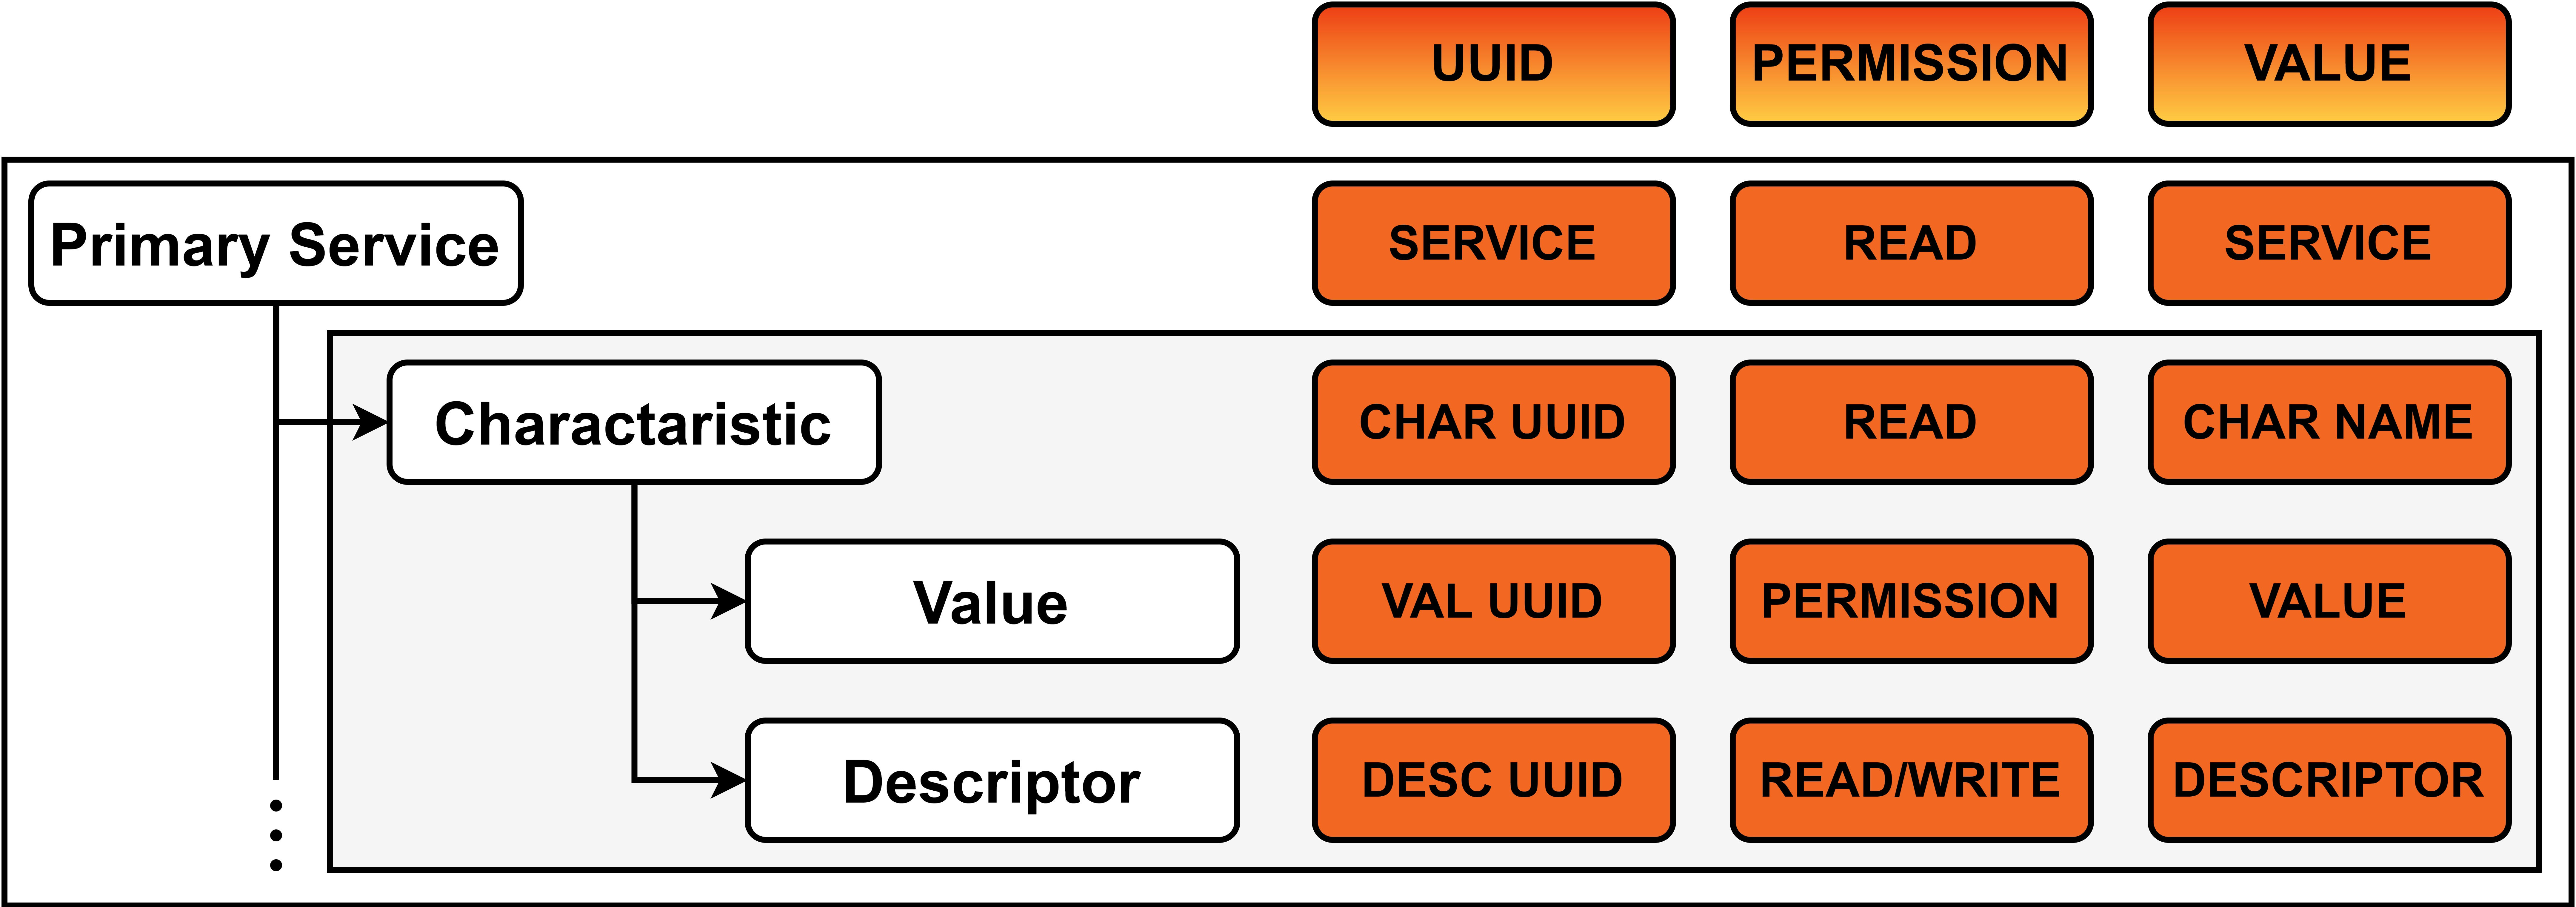
\includegraphics[width = 0.9 \textwidth]{BLEservice.jpg}
		\caption{\ac{ble} Specification Structure}
		\label{fig:serv}
		\citep[Adapted from ][chap.~4]{Townsend:2014}
	\end{center}
\end{figure}

\vspace{-0.7 cm}

When a connection with the Zwift application is established over \ac{ble}, the \ac{ftms} service is implemented for communicating with training platforms and was thus investigated in further detail.

\subsubsection{\ac{ftms} Protocol}\label{sec:ftms}

As mentioned in section \ref{sec:ble}, \acf{ftms} is a service specification under the \acf{gatt} with a \ac{uuid} of 0x1826. The \ac{ftms} service specification contains 15 different characteristics, of which 7 are related to cycling training platforms. These characteristics are listed in table \ref{tab:ftmsft}, along with their \acp{uuid} and required properties. \cite[section ~4.9]{BLSIG:2017}.

\footnotetext[1]{\acl{fm}}

\begin{table}[H]
	\renewcommand{\arraystretch}{\tablestretch}
	\centering
	\caption{\ac{ftms} Characteristics for Bicycle Training Platforms}
	\citep{Huawei:2022}
	\begin{tabularx}{\textwidth}{>{\raggedright}p{3cm} >{\raggedright}X >{\raggedright}p{2.3cm} p{1.3cm}}
		\toprule
		Characteristic                               & Description                             & Properties       & \acs{uuid} \\
		\midrule
		Indoor Bike Data                             & Reports live workout data               & Notify           & 0x2AD2     \\
		Training Status                              & Reports training device status          & Read / Notify    & 0x2AD3     \\
		Speed Range                                  & Reports supported speed range           & Read             & 0x2AD4     \\
		Power Range                                  & Reports supported power range           & Read             & 0x2AD8     \\
		\acs{fm}\footnote[1]{\acf{fm}} Control Point & Controls fitness machine status         & Write / Indicate & 0x2AD9     \\
		\acs{fm}\footnote[1]{\acf{fm}} Status        & Reports changes in workout status       & Notify           & 0x2ADA     \\
		\acs{fm}\footnote[1]{\acf{fm}} Feature       & Describes device supported capabilities & Read             & 0x2ACC     \\
		\bottomrule
	\end{tabularx}
	\label{tab:ftmsft}
\end{table}

\vspace{-0.5 cm}

\subsubsection{\ac{sim} mode}
\label{sec:sim}

\color{red}

This mode is defined in the \ac{ftms} documentation, and needs Control Permission to be activated. Once the mode is activated, the trainer will receive parameter arrays with the data shown in Table \ref{tab:sim} below to determine the required resistance level.

\begin{table}[H]
	\renewcommand{\arraystretch}{\tablestretch}
	\centering
	\caption{\ac{sim} Mode Parameter Data}
	\begin{tabularx}{\textwidth}{>{\raggedright\arraybackslash}X >{\centering\arraybackslash}p{2cm} >{\centering\arraybackslash}p{1cm} >{\raggedleft\arraybackslash}p{2cm}}
		\toprule
		Parameter  & Unit                       & Size   & Resolution \\
		\midrule
		Wind Speed & \SI{}{\meter\per\second}   & 16 bit & 0.001      \\
		Grade      & \SI{}{\percent}            & 16 bit & 0.01       \\
		\ac{crr}   &                            & 8 bits & 0.0001     \\
		\ac{cw}    & \SI{}{\kilogram\per\meter} & 8 bits & 0.01       \\
		\bottomrule
	\end{tabularx}
	\label{tab:sim}
\end{table}

\vspace{-0.5 cm}

The \textit{Grade} indicates the gradient of the road that the avatar is travelling on. The \text{\ac{crr}} is determined by the road surface and wheel type of the avatar in the game, where the \textit{\ac{cw}} is determined by the player's weight and height, and can then be reduced by in-game events such as equipment selection and drafting behind other avatars when this feature is active. Currently Zwift does not utilize the \textit{Wind Speed} parameter.

\color{black}

\vspace{-0.5cm}

\newpage

\section{Existing Trainer Technology}
\label{sec:train}

There are four types of bicycle trainers that are commonly used for indoor cycling. \textit{Roller trainers} consists of roller drums on which a bicycle's wheels may spin freely (\ref{fig:roller}). \textit{Wheel-on resistance trainers} (aka. turbo trainers) allow for the bicycle to be fixed into a stationary position with some resistance applied to the rotation of the rear wheel (\ref{fig:wheelon}). \textit{Direct-drive trainers} are similar to wheel-on trainers where the bicycle is fixed in a stationary position, but with at least the rear wheel removed. This allows the resistance to be applied directly to the bicycle's drivetrain (\ref{fig:directdrive}). The fourth type consists of a completely independent platform that does not require a bicycle to operate. \citep{Alff:2011}

\vspace{-0.5cm}

\begin{figure}[H]
	\centering
	\begin{subfigure}{.3\textwidth}
		\centering
		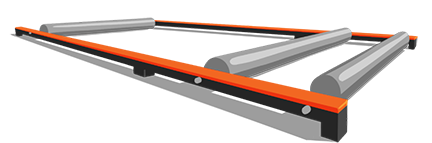
\includegraphics[width=\linewidth]{Roller.jpg}
		\caption{Roller Trainer}
		\label{fig:roller}
	\end{subfigure}
	\hfill
	\begin{subfigure}{.3\textwidth}
		\centering
		
\includegraphics[width=\linewidth]{Trainer_WheelOn.jpg}
		\caption{Wheel On Trainer}
		\label{fig:wheelon}
	\end{subfigure}
	\hfill
	\begin{subfigure}{.3\textwidth}
		\centering
		
\includegraphics[width=\linewidth]{Trainer_DirectDrive.jpg}
		\caption{Direct Drive Trainer}
		\label{fig:directdrive}
	\end{subfigure}
	\caption{Bicycle Dimensions}
	\label{fig:trainers}
	\citep{Zwift:2022}
\end{figure}

\newpage

\section{Bicycle Specifications}
\label{sec:specs}
% Section showing expected bicycle specifications of most popular models
The two most common types of bicycles that are expected to be used on the trainer are \acp{mtb} and road bicycles. For the design of a bike trainer, the relevant dimensions to consider are the wheelbase wheel diameter and weight as illustrated in Figure \ref{fig:bikeDim}.

\begin{figure}[H]
	\centering
	\begin{subfigure}{.5\textwidth}
		\centering
		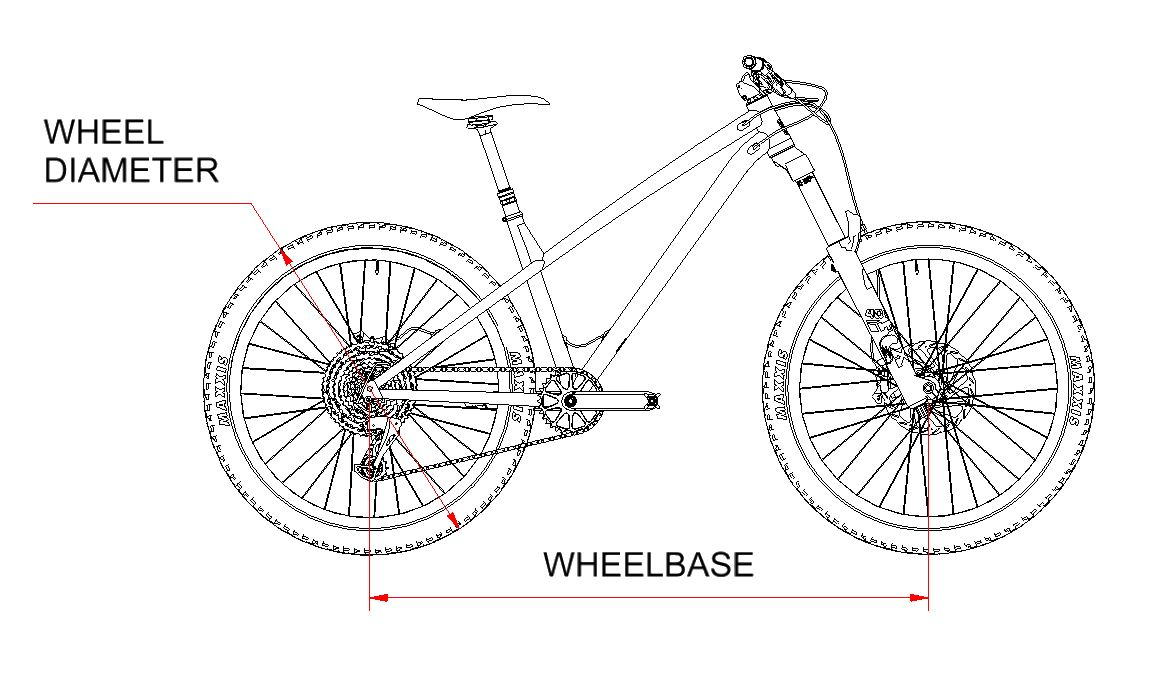
\includegraphics[width=\linewidth]{measureMTB.jpg}
		\caption{\ac{mtb} \citep[model by:][]{Pratama:2021}}
		\label{fig:sub1}
	\end{subfigure}%
	\begin{subfigure}{.5\textwidth}
		\centering
		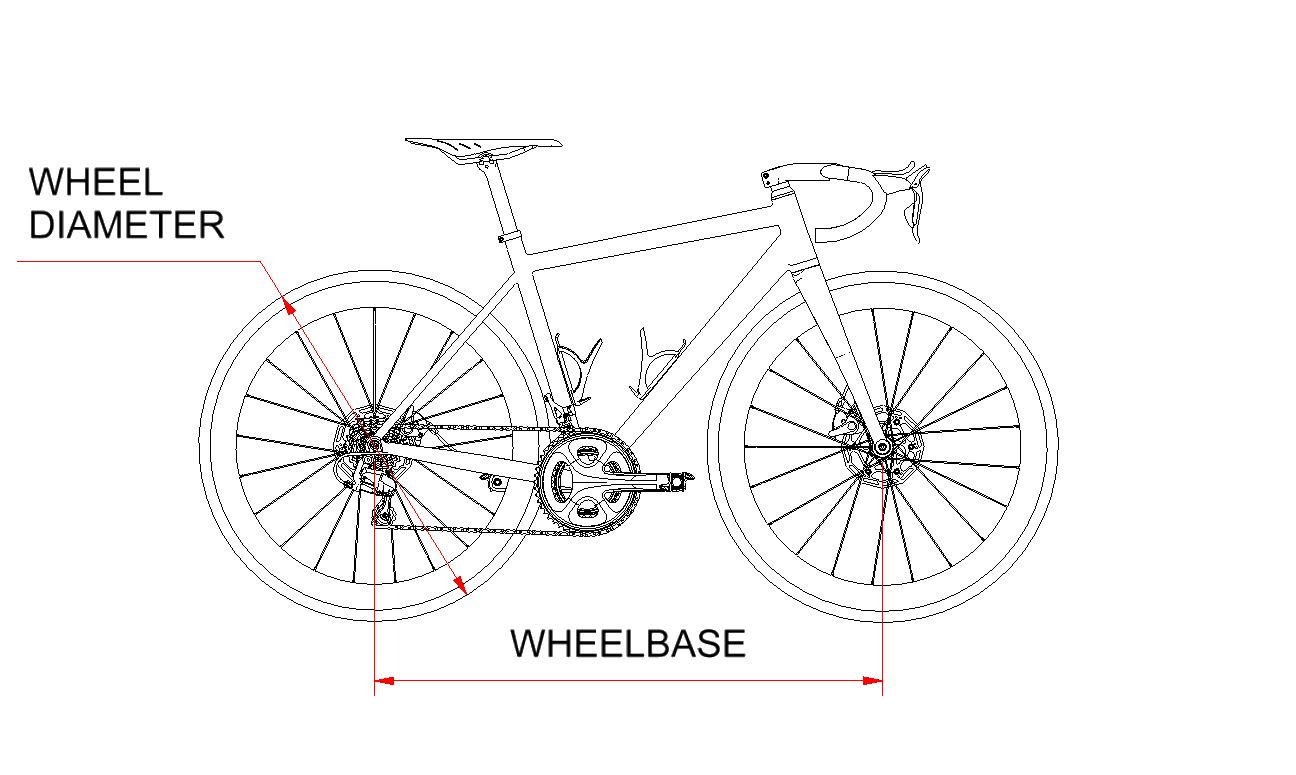
\includegraphics[width=\linewidth]{measureRoad.jpg}
		\caption{Road Bicycle \citep[model by:][]{Morozev:2017}}
		\label{fig:sub2}
	\end{subfigure}
	\caption{Bicycle Dimensions}
	\label{fig:bikeDim}
\end{figure}

\vspace{-0.6 cm}

Although these dimensions vary between brands, models and sizes, a general overview of common dimensions can be found by comparing the dimensions of the largest and smallest size offerings from the best selling models in each category in Table \ref{tab:bikes}. \citep{Lin:2021} 

\begin{table}[H]
	\renewcommand{\arraystretch}{\tablestretch}
	\centering
	\caption{Best Selling Road and \ac{mtb} specifications}
	\citep{Geometry:2022}
	\begin{tabularx}{\textwidth}{p{2.6cm} X Xp{0.05cm} p{2.6cm} X X}
		\toprule
		Road Bike           & \multicolumn{2}{c}{Wheelbase} &                         & \ac{mtb} & \multicolumn{2}{c}{Wheelbase}                                                     \\
		                    & Smallest                      & Largest                 &          &                               & Smallest                & Largest                 \\
		\midrule
		Specialized Tarmac  & \SI{969}{\milli\meter}        & \SI{1012}{\milli\meter} &          & Specialized Epic              & \SI{1116}{\milli\meter} & \SI{1211}{\milli\meter} \\
		Specialized Roubaix & \SI{981}{\milli\meter}        & \SI{1024}{\milli\meter} &          & Trek Fuel EX                  & \SI{1144}{\milli\meter} & \SI{1323}{\milli\meter} \\
		Cervelo R3          & \SI{971}{\milli\meter}        & \SI{1024}{\milli\meter} &          & Specialized Stumpjumper       & \SI{1152}{\milli\meter} & \SI{1302}{\milli\meter} \\
		\bottomrule
	\end{tabularx}
	\label{tab:bikes}
\end{table}

The most common wheel diameter sizes for both road bicycles and \ac{mtb} are 27.5" (aka. 650c) and 29" (aka. 700c). The 27.5" and 29" refer to the diameter of the rim in inches, where the 650c and 700c refer to the typical diameter with a tyre on in \si{\milli\meter}. The dimension that is relevant to the design of a bicycle training platform is the diameter with the wheel on, and will thus commonly range between \SI{650}{\milli\meter} and \SI{700}{\milli\meter}. \citep{Montague:2019}

\section{Eddy Current Brake}
% Section on Eddy Current Brake

\subsubsection{Working Principle}

An \acf{ecb} is a contactless braking device that consists of a stationary magnetic flux source and a moving conductor. The magnetic flux source can be from either permanent magnets or electromagnets, and the conductor typically takes the form of a rail, drum or disk. As the conductor moves through the stationary magnetic flux, it experiences a time-varying magnetic flux density. According to Lenz's law (Equation \ref{eq:lenz}), this time-varying magnetic flux density $\frac{\delta\vec{B}}{\delta t}$ results in an electric field $\vec{\ac{E}}$.

\begin{equation}
	\nabla \times \vec{\ac{E}} = \frac{\delta\vec{\ac{B}}}{\delta t}
	\label{eq:lenz}
\end{equation}

According to Ohm's Law (Equation \ref{eq:ohm2}), this electric field results in circulating currents $\vec{\ac{J}}$ within the conductor with conductance \acs{condDisk}.

\begin{equation}
	\vec{\ac{J}} = \ac{condDisk} \cdot \vec{\ac{E}}
	\label{eq:ohm2}
\end{equation}

These circulating currents are called "Eddy-currents", and the interaction of these eddy-currents with the flux density results in a force $\vec{\acs{F}}$ that opposes the motion: \citep{Gay:2005}

\begin{equation}
	\vec{\ac{F}} = \vec{\ac{J}} \times \vec{\ac{B}}
	\label{eq:force}
\end{equation}

\subsubsection{Mathematical Model}

\cite{Smythe:1942} first proposed a mathematical model that includes two distinct torque regions. Below the critical speed, the torque vs. speed relation is approximately linear, and the high speed region approaches some constant. This model was the further expanded and improved by \cite{Smythe:1950}.

\cite{Wouterse:1991} proposed a model for the induced torque at the critical speed, as the torque in this region cannot be expressed simply as a function of magnetic flux and disk speed. 

\cite{Baum:2016} proposed a model for the performance of an \ac{ecb} with two pole pairs on a rotating conductive disk. This model builds on the work of \cite{Smythe:1950} and \cite{Wouterse:1991} to take into account the saturation of the disk and the demagnetization effect of the induced magnetic flux on the magnets. This results in Equation~\ref{eq:low} for the low speed region and Equation~\ref{eq:high} for the high speed region. The critical speed is found by equating these two equations.

\begin{equation}
	\ac{F}_{Low Speed} = n_{pairs} \cdot \ac{condDisk} \cdot \ac{v} \cdot {\ac{B}_0}^2 \cdot A_{magnet} \cdot t_{disk}
	\label{eq:low}
\end{equation}

\begin{equation}
	\ac{F}_{High Speed} = n_{pairs} \cdot \frac{1}{\ac{v}} \cdot t_{magnet}^2 \cdot \frac{\ac{B}_0^2}{\acs{permeability}_0^2} \cdot \frac{1}{\ac{condDisk}} \cdot \frac{2 D_{magnet}}{t_{disk} \cdot \delta d_{magnets}}
	\label{eq:high}
\end{equation}

\begin{figure}[H]
	\begin{center}
		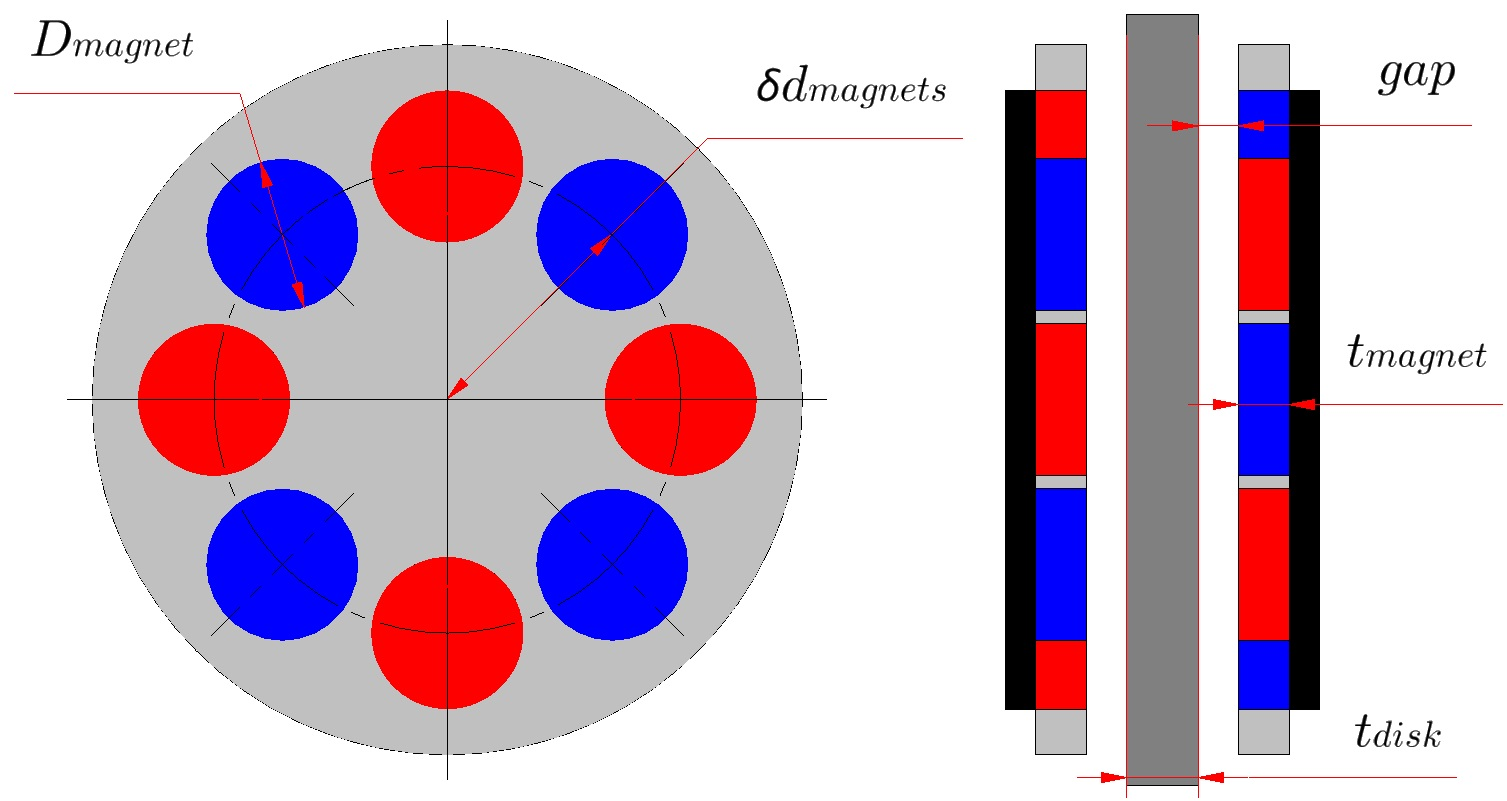
\includegraphics[width=0.6\textwidth]{Brake Layout.jpg}
		\caption{Eddy Current Brake Dimensions (To be changed ...)}
		\label{fig:EB}
	\end{center}
\end{figure}

\newpage

\section{Sensor Technology}
% Tachometer
% Torque Transducer

\newpage

% \section{Conclusion}
% Section summerizing the literature review
